%% Manuscript in the Wiley New Journal Design v5 template (WileyNJDv5.cls).
%% Put the template files (WileyNJDv5.cls, *.bst, *.sty and the Fonts folder) in this folder.
%% Reference style: Vancouver (numbered). Compile with pdfLaTeX or XeLaTeX:  pdflatex main && bibtex main && pdflatex main && pdflatex main
%% Figures are read from ../figures and tables from ../tables, both generated from the result
%% files by scripts/make_figures.py and scripts/make_tables.py.
% Compatibility with TeX Live 2024 and later (newer etex.sty lacks \reserveinserts, which the class calls)
\providecommand\reserveinserts[1]{}
\documentclass[VANCOUVER,Times1COL]{WileyNJDv5}

\usepackage{booktabs,multirow}
\usepackage{algorithm}
\usepackage{algpseudocode}
\graphicspath{{figures/}{../figures/}}
% tables: works with tables/ next to main.tex (Overleaf) or ../tables (repository layout)
\newcommand{\inputtable}[1]{\IfFileExists{tables/#1.tex}{\input{tables/#1}}{\input{../tables/#1}}}

\articletype{Research Article}
\received{Date Month Year}
\revised{Date Month Year}
\accepted{Date Month Year}
\journal{Journal}
\volume{00}
\copyyear{2026}
\startpage{1}
\raggedbottom

\setcounter{secnumdepth}{3}
\begin{document}

\title{Lesion-level leakage and site-level reliability in Fed-ISIC2019: an audit of federated skin lesion classification}

\author[1]{Abu Jafar Sisty}
\author[1]{Author Name} % TODO: author 2 name (change [1] if a different affiliation)
\author[1]{Author Name} % TODO: author 3 name
\author[1]{Author Name} % TODO: author 4 name
\authormark{SISTY \textsc{et al.}}
\titlemark{LESION-LEVEL LEAKAGE AND SITE-LEVEL RELIABILITY IN FED-ISIC2019}

\address[1]{\orgname{American International University-Bangladesh}, \orgaddress{\street{408/1 Kuratoli, Khilkhet}, \city{Dhaka} \postcode{1229}, \country{Bangladesh}}}
\corres{Corresponding author: Abu Jafar Sisty. \email{22-49133-3@student.aiub.edu}}

\abstract[Abstract]{\textbf{Background:} Fed-ISIC2019 is a widely used benchmark for federated skin
lesion classification. Its split assigns images rather than lesions to training and test sets, so images
of one lesion can appear on both sides, and the reliability of probabilities and prediction sets at
individual sites is rarely reported.
\textbf{Methods:} We audited the benchmark's six acquisition-source clients (23,247 dermoscopy images)
with image-level and lesion-grouped splits (three to five seeds per experiment), three encoder
configurations (fine-tuned and frozen EfficientNet-B0, frozen PanDerm) and up to eight federated,
personalized, centralized and local methods. We measured the apparent accuracy gain on leaked test images,
ran a randomized sibling-exposure experiment on fixed test images, and evaluated method rankings,
calibration and federated conformal coverage per client, on held-out clients and on smartphone images
(PAD-UFES-20). We also evaluated EB-ShrinkFCP, an empirical-Bayes rule for per-client conformal
thresholds. Confirmatory tests followed a version-controlled protocol fixed before the corresponding runs.
\textbf{Results:} In the official split, 0.1--93\% of each client's test images had a sibling image in
training. For FedAvg, balanced accuracy on the full image-level test set exceeded a standardized
new-lesion estimate by 8.1 points (95\% CI 4.7--11.2), and by up to 16.2 points for centralized
training. In a randomized crossover on fixed test images, having a sibling image in training raised balanced accuracy by 9.1 points (5.5--12.3) for FedAvg and by up to 28.8 points for local training. With frozen foundation-model features, method rankings were unrelated across split
types (Kendall's $\tau_b=0.05$). Calibration varied more between clients than between methods, and an apparent ECE gap between leaked and new lesions disappeared after matching sample size and composition. A global conformal threshold left some clients at 0.72--0.83
mean coverage (target 0.90). EB-ShrinkFCP kept mean client coverage near 0.90 and met its pre-specified
criterion for one of two encoders (worst-client 10th-percentile coverage +2.3 points, 0.8--3.9), so the
joint criterion was not met; a fixed shrinkage rule failed. On smartphone images, transferred coverage
fell to 0.60--0.67.
\textbf{Conclusions:} Federated dermatology benchmarks should use lesion-grouped splits and report
calibration and conformal coverage per client, with the coverage target stated. Splits, code, predictions
and the protocol history are released.}

\keywords{federated learning, data leakage, skin lesion classification, calibration, conformal prediction, benchmarking}


\maketitle

\renewcommand\thefootnote{}
\footnotetext{\textbf{Abbreviations:} BA, balanced accuracy; CI, confidence interval; ECE, expected calibration error;
FL, federated learning; LAC, least ambiguous set-valued classifier; LOCO, leave-one-client-out; q10, 10th percentile
of coverage over calibration draws.}
\renewcommand\thefootnote{\fnsymbol{footnote}}
\setcounter{footnote}{1}

% ============================================================== 1. Introduction
\section{Introduction}
\label{sec:intro}

Deep learning classifiers for dermoscopy images can match dermatologists on curated test sets
\cite{esteva2017dermatologist}, but their performance can drop on
data that differ from the training distribution \cite{daneshjou2022disparities}, and robust models need
large and diverse training data that are held by separate institutions. Privacy regulation and
institutional policy often prevent pooling such data, which has made federated learning (FL), in which
sites train a shared model without exchanging images, a central approach for multi-institutional medical
imaging \cite{rieke2020future,sheller2020federated,dayan2021exam}. Claims about FL
for clinical use, however, rest on benchmarks, and a benchmark is informative only if its evaluation
reflects the situation of a new lesion at a participating or a new site.

For skin lesions, Fed-ISIC2019, the dermoscopy benchmark of the FLamby suite \cite{flamby2022}, is
widely used. Its six clients correspond to acquisition sources of the ISIC 2019 challenge data
\cite{codella2018isic,tschandl2018ham,combalia2019bcn} and differ in size, class mix and imaging
device. Federated and personalized methods are compared on its fixed split, and the reported differences
between them are often a few points of balanced accuracy \cite{flamby2022,tavakoli2024fendafl}.

The benchmark split assigns individual images rather than lesions to the training and test sets. Many
lesions in the underlying collections were photographed several times, for example at follow-up visits or
with different magnifications. An image-level split therefore places correlated views of one lesion on
both sides (Figure~\ref{fig:leakage}a), so the test set partly measures recognition of lesions seen in
training rather than diagnosis of new ones. Such leakage is a known cause of over-optimistic results in
machine learning \cite{kapoor2023leakage,varoquaux2022failures}. In dermatology, duplicates and
problematic partitions have been documented in centralized datasets
\cite{cassidy2022isic,groger2023reliable,abhishek2025dermamnist}, and subject-level splitting has
inflated accuracy in histopathology and brain MRI \cite{bussola2021tiles,yagis2021leakage}. We found no
study that quantifies lesion-level leakage per client in Fed-ISIC2019 or examines its consequences for
federated method comparisons, calibration and conformal coverage. Because clients differ in size and
acquisition protocol, leakage need not be uniform: in the official Fed-ISIC2019 split, 93\% of one
client's test images have a sibling image in training, compared with 0.1\% in another. Leakage may
therefore distort not only absolute accuracy but also comparisons between methods that fit client-level
data to different degrees, such as local and personalized models.

A second gap concerns reliability at the level of the individual site. FL studies usually report a
single accuracy over the pooled test set, whereas a clinician needs calibrated probabilities
\cite{guo2017calibration} and, ideally, prediction sets whose error rate is controlled at their own
site. Conformal prediction provides sets with distribution-free marginal coverage under exchangeability
\cite{vovk2005algorithmic,angelopoulos2023gentle}, and federated variants target coverage on the
mixture of clients, under label shift, or for personalized and group-defined targets
\cite{lu2023fcp,humbert2023oneshot,plassier2023labelshift,min2025pfcp,wen2026gcfcp}. A
threshold computed from pooled scores can under-cover individual clients while meeting its mixture
target, and a threshold computed from a small client's own data controls coverage on average but varies
strongly between calibration samples. How these effects play out on the Fed-ISIC2019 clients, how they
interact with leakage and with the repeated images of one lesion, and how they change on unseen clients
or images from another device has, to our knowledge, not been reported.

In this study we audit federated skin lesion classification on Fed-ISIC2019 with image-level and
lesion-grouped splits. We train up to eight federated, personalized, centralized and local methods with
three encoder configurations (a fully fine-tuned convolutional network, the same network frozen, and a
frozen dermatology foundation model) and evaluate accuracy, method rankings, calibration and conformal
coverage overall and per client, on held-out clients and on smartphone images. Confirmatory analyses
followed a version-controlled protocol fixed before the corresponding runs, and we report the tests that
failed alongside those that succeeded. Our contributions are:
\begin{enumerate}
  \item A per-client audit of lesion-level leakage in Fed-ISIC2019, of the apparent accuracy gain it
    produces, and of its consequences for method rankings, calibration and conformal coverage, together
    with a randomized sibling-exposure experiment that estimates the effect of leakage on fixed test
    images.
  \item Evidence that leakage inflates accuracy also with frozen encoders, including a dermatology
    foundation model, and randomized and capacity-matched experiments showing that its size grows with how
    closely a classifier fits its training lesions, not with personalization as such.
  \item A per-client analysis of federated conformal calibration that separates mixture from per-client
    coverage and accounts for repeated images of one lesion, and EB-ShrinkFCP, an empirical-Bayes
    shrinkage rule for per-client thresholds that met its pre-specified criterion for one of two encoders.
  \item Lesion-grouped splits, code, predictions and the complete protocol history, released to support
    leakage-free federated benchmarking.
\end{enumerate}

The remainder of the paper is organized as follows. Section~\ref{sec:related} reviews related work,
Section~\ref{sec:methods} describes the data, models and analyses, Section~\ref{sec:results} reports the
results by research question, Section~\ref{sec:discussion} discusses their implications and limitations,
and Section~\ref{sec:conclusion} concludes.

\begin{figure*}[!t]
  \centering
  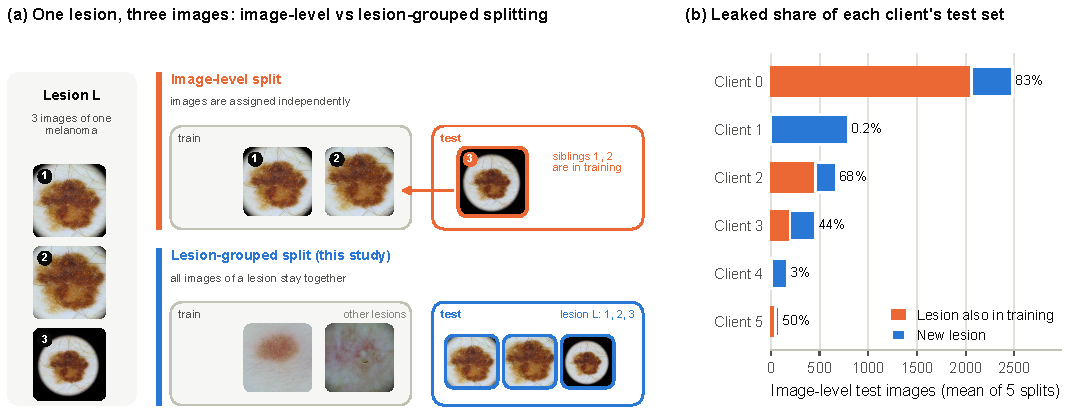
\includegraphics[width=\textwidth]{Fig1_design_leakage}
  \caption{Lesion-level leakage in Fed-ISIC2019. (a) The three images of one melanoma of client~0 (lesion
  BCN\_0000057; images ISIC\_0057997, ISIC\_0065360 and ISIC\_0068295, all sharing this identifier in the
  ISIC 2019 metadata). In the official FLamby split, the first two are training images and the third is a
  test image; under a lesion-grouped split, all images of a lesion stay on one side. (b) Image-level test
  images per client that are leaked (their lesion also has images in training) or new; percentages give
  the leakage rate as the mean over five image-level re-splits (the official split is reported in
  Table~\ref{tab:dataset}). Images: ISIC 2019 (CC-BY-NC 4.0).}
  \label{fig:leakage}
\end{figure*}

% ============================================================== 2. Related work
\section{Related work}
\label{sec:related}

\subsection{Federated learning for medical imaging and dermatology}

FedAvg \cite{mcmahan2017fedavg} trains a global model by averaging locally updated parameters. Because
clients hold non-identically distributed data, many variants correct client drift, for example FedProx
with a proximal term \cite{li2020fedprox} and SCAFFOLD with control variates
\cite{karimireddy2020scaffold}, or personalize parts of the model, for example local batch-normalization
layers in FedBN \cite{li2021fedbn}, local classification layers in FedPer \cite{arivazhagan2019fedper},
or local fine-tuning of the global model; surveys review these
families \cite{kairouz2021advances,tan2023pfl}. In medical imaging, FL has been studied for brain tumor
segmentation, chest imaging and outcome prediction across hospitals
\cite{sheller2020federated,dayan2021exam}, and its promises and pitfalls have been reviewed
\cite{rieke2020future}. FLamby introduced Fed-ISIC2019 as a cross-silo dermatology
benchmark with clients defined by acquisition source \cite{flamby2022}, and Tavakoli et al.\ used it to
compare personalized methods on heterogeneous clinical data \cite{tavakoli2024fendafl}. Both evaluations
use FLamby's fixed image-level split. Dermatology foundation models such as PanDerm, pretrained on
millions of skin images, now offer strong frozen features \cite{yan2025panderm}; how leakage affects
comparisons on such features has not been examined.

\subsection{Data leakage and evaluation pitfalls in medical imaging}

Leakage, in which information about the test data reaches the training process, is a widespread cause
of irreproducible results in machine-learning-based science \cite{kapoor2023leakage}. In medical imaging
it often arises when images from the same subject appear in training and test sets: splitting
histopathology slides at the tile level \cite{bussola2021tiles} and brain MRI volumes at the slice level
\cite{yagis2021leakage} markedly overestimated classification performance compared with subject-level
splits. Related failure modes include confounding by acquisition site \cite{zech2018confounding} and shortcut
learning \cite{degrave2021shortcuts}, both of which
can make held-out performance unrepresentative \cite{roberts2021pitfalls,varoquaux2022failures}. In
dermatology, Cassidy et al.\ found duplicates across the yearly ISIC releases and proposed curated
training and test sets \cite{cassidy2022isic}; Gr\"oger et al.\ removed near-duplicates and other
problems from six dermatology evaluation benchmarks \cite{groger2023reliable}; and Abhishek et al.\ showed
that duplicates leaked across the splits of DermaMNIST and Fitzpatrick17k and released corrected
partitions \cite{abhishek2025dermamnist}. These studies establish that dermatology benchmarks can contain
leakage; they concern centralized datasets and accuracy. What we add is the per-client distribution of
lesion-level leakage in a federated benchmark, a randomized estimate of its effect, and its consequences
for method rankings, calibration and conformal coverage.

\subsection{Calibration of medical image classifiers}

Modern neural networks are often over-confident \cite{guo2017calibration}. Calibration is typically
measured with the expected calibration error \cite{naeini2015ece}, class-wise variants
\cite{kull2019beyond}, the negative log-likelihood and the Brier score \cite{brier1950}, and improved post
hoc by temperature scaling \cite{guo2017calibration} or by approximate Bayesian and ensemble methods
\cite{gal2016dropout}. Calibration degrades under dataset shift
\cite{ovadia2019trust} and depends on architecture and training \cite{minderer2021revisiting}, and it has
been studied in medical imaging, for example for segmentation networks \cite{mehrtash2020confidence}. The question we
address is narrower: how calibration varies across the clients of Fed-ISIC2019 and whether a test set with
lesion-level leakage changes calibration estimates and the effect of temperature scaling.

\subsection{Conformal prediction in federated settings}

Split conformal prediction turns any classifier into a set-valued predictor with marginal coverage of at
least $1-\alpha$ when calibration and test points are exchangeable
\cite{vovk2005algorithmic,angelopoulos2023gentle}; common scores for classification
are LAC \cite{sadinle2019lac} and APS \cite{romano2020aps}. Coverage can fail under
covariate or label shift \cite{tibshirani2019covariate,podkopaev2021labelshift,barber2023beyond}, can
differ between subgroups \cite{lu2022fair}, and needs adapted arguments when observations are grouped,
as are repeated images of one lesion \cite{dunn2022hierarchical,lee2023hierarchical}. Several coverage
targets must be distinguished: marginal coverage on the mixture of clients, coverage for each client,
coverage for each class, and the probability over calibration samples that coverage falls short.
Federated conformal methods compute thresholds without pooling scores: Lu et al.\ derived a federated
quantile with a guarantee on the mixture of clients under partial exchangeability
\cite{lu2023fcp}, Humbert et al.\ proposed a one-shot quantile-of-quantiles scheme
\cite{humbert2023oneshot}, Plassier et al.\ addressed label shift between clients
\cite{plassier2023labelshift}, Min et al.\ personalized conformal sets through localization
\cite{min2025pfcp}, and Wen et al.\ targeted group-conditional coverage \cite{wen2026gcfcp}. A method can
meet its mixture target while under-covering a particular client; it is not disproved by failing a per-client objective it was not designed for, but it is insufficient for site-level use. Per-client thresholds avoid that bias
but are noisy for small clients. Shrinking noisy estimates toward a common mean is a classical idea,
from normal-means empirical Bayes \cite{efron1975stein} to random-effects meta-analysis
\cite{dersimonian1986meta}. EB-ShrinkFCP applies it to per-client conformal quantiles with only two
numbers per client; its methodological novelty is limited to this application, and we evaluate it
empirically on real clients, on held-out clients and against client-wise, global, FCP and
label-shift-weighted thresholds.

% ============================================================== 3. Materials and methods
\section{Materials and methods}
\label{sec:methods}

\subsection{Study overview and research questions}
\label{sec:overview}

Fig.~\ref{fig:framework} summarizes the study. We trained federated, personalized, centralized and
local models on the six clients of Fed-ISIC2019, once on image-level splits (the common practice) and
once on lesion-grouped splits, and evaluated accuracy, calibration and conformal coverage overall and per
client. Four research questions organize the methods, results and discussion:

\begin{description}
\item[RQ1] With a lesion-grouped split, how reliable are federated accuracy, calibration and conformal
  coverage overall, per client, on clients unseen in training, and under a shift to smartphone images?
\item[RQ2] How unevenly is lesion leakage distributed across the Fed-ISIC2019 clients, and how much does
  it change apparent accuracy, method rankings, calibration and conformal coverage?
\item[RQ3] Does personalization improve per-client results under a lesion-grouped split, and do local
  and personalized models show the largest apparent gain from leakage (hypothesis H3b)?
\item[RQ4] Can a client-specific conformal threshold that borrows strength from the other clients
  reduce low-coverage calibration draws in small clients without enlarging prediction sets?
\end{description}

The experiments were: E0, reproduction of the published benchmark on the official split; E1,
image-level versus lesion-grouped splits for three encoder configurations; E2, eight training methods on
both split types; E3, calibration; E5, federated conformal prediction on in-federation models; E6,
leave-one-client-out (LOCO) models and a smartphone-image stress test; E7, personalized models and the
final test of H3b; E8, a randomized sibling-exposure experiment on fixed test images; and E9,
capacity-matched classifier heads for model~B. The optional experiment E4 was not run. Seeds differed
between experiments (Supplementary~S10 gives the full run matrix): three for E0, E1, E6 and E8, five for E2, E7
and E9. Confirmatory tests followed the protocol version that was fixed before the corresponding runs
(Section~\ref{sec:prereg}); all other analyses are labelled secondary, post hoc or exploratory.

\begin{figure*}[!t]
  \centering
  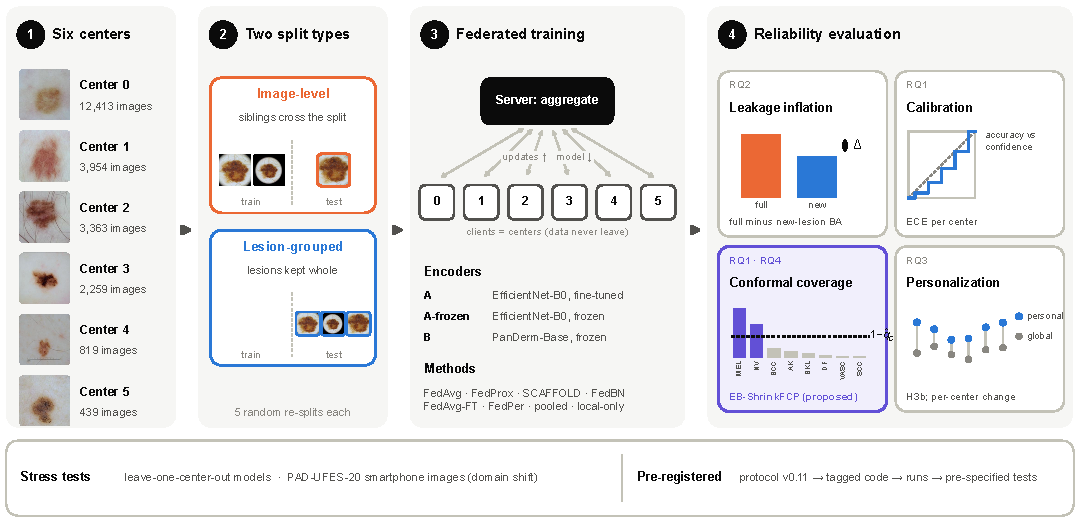
\includegraphics[width=\textwidth]{Fig2_framework}
  \caption{Study framework. (1) Six Fed-ISIC2019 clients (acquisition sources) with one example image
  each. (2) Models are trained and evaluated on image-level splits, in which images of one lesion can
  fall on both sides, and on lesion-grouped splits, in which they cannot (three to five random re-splits
  of each type, depending on the experiment; Supplementary~S10). (3) Simulated federated training with three
  encoder configurations and up to eight methods: images stay with their client during federated
  training, while the centralized baseline pools them. (4) Four evaluation questions; the proposed
  EB-ShrinkFCP is highlighted. Bottom: stress tests and the version-controlled protocol. Images: ISIC
  2019 (CC-BY-NC 4.0).}
  \label{fig:framework}
\end{figure*}

\subsection{Datasets}
\label{sec:data}

\paragraph{Fed-ISIC2019} We used the Fed-ISIC2019 benchmark of FLamby \cite{flamby2022} (commit
\texttt{edacf54}): 23,247 dermoscopy images from the ISIC 2019 challenge
\cite{codella2018isic,tschandl2018ham,combalia2019bcn}, labelled with eight diagnostic classes
(melanoma, MEL; melanocytic nevus, NV; basal cell carcinoma, BCC; actinic keratosis, AK; benign
keratosis, BKL; dermatofibroma, DF; vascular lesion, VASC; squamous cell carcinoma, SCC). FLamby defines
six clients by acquisition source (Table~\ref{tab:dataset}): BCN20000 (client~0), MSK (client~4) and four
HAM10000 subsets, three of which (clients 1, 2 and 5) come from one institution in Vienna with different
acquisition devices. FLamby calls the clients ``centers''; we call them clients because they are acquisition sources rather
than six independent hospitals. Images were preprocessed with FLamby's procedure (shorter
edge resized to 224 pixels, color constancy with power 6).

Lesion identifiers were taken from the HAM10000 metadata (clients 1, 2, 3 and 5) and the ISIC 2019
metadata (clients 0 and 4). All 23,247 images have an identifier; none equals its image name, no lesion
carries two diagnoses, and the data contain 11,847 lesions. Nine lesions have images in two clients
(clients 1 and 2, both from the Vienna institution), which is why the per-client lesion counts in
Table~\ref{tab:dataset} sum to 11,856. The number of images per lesion ranges from one to 31 (median 1;
3.47 on average in client~0). Patient identifiers are not available for Fed-ISIC2019, so our splits are
lesion-disjoint but not necessarily patient-disjoint. Supplementary~S1 gives the per-client and per-class
counts and the identifier checks.

\inputtable{Table1_dataset}

\paragraph{PAD-UFES-20} As a domain-shift stress test we used PAD-UFES-20 \cite{pacheco2020pad}:
2,298 clinical photographs taken with smartphones (not dermoscopy) from 1,373 patients. Its six
diagnoses were mapped to the Fed-ISIC2019 classes (MEL$\to$MEL, NEV$\to$NV, BCC$\to$BCC,
ACK$\to$AK, SEK$\to$BKL, SCC$\to$SCC). This is a closed-set transfer: model probabilities were
restricted to the six shared classes and renormalized before any metric or conformal threshold was
computed, on the source and the target data alike. Lesion numbers in the PAD-UFES-20 metadata are
reused across patients (250 numbers occur under two patient identifiers, mostly with different
diagnoses; the pair of patient and lesion number identifies 1,891 lesions), so all PAD-UFES-20 analyses
were grouped by patient. No model was trained or fine-tuned on PAD-UFES-20.

\subsection{Data splits}
\label{sec:splits}

Three kinds of split were used (files, checksums and realized sizes are in the code repository and
Supplementary~S1).
\emph{Official}: FLamby's fixed image-level split, used to reproduce published results (E0) and to
report the leakage of the benchmark as distributed.
\emph{Image-level} re-splits: 20\% of each client's images form the test set, stratified by class,
irrespective of lesion.
\emph{Lesion-grouped} re-splits: 20\% of each client's lesions, with all their images, form the test set,
under class quotas; the nine lesions with images in two clients were always kept in training. Because the
two split types draw 20\% of images and 20\% of lesions respectively, their training sets differ by less
than 1\% in images (about 16,700--16,800) but not in lesions (about 9,350 versus 8,500), and their test
sets differ in composition (Supplementary~S1). From E1 onwards, 10\% of each client's training lesions
were moved to a validation fold, grouped by lesion in both split types; the validation fold was used only
for temperature scaling. In the lesion-grouped splits no lesion occurs in more than one of training,
validation and test. In the image-level splits this holds for training and validation, but 6.5\% of the
test images belong to a lesion that is in the validation fold and not in training; these images were
counted as new (they were not used for training) and are examined in a sensitivity analysis. The split
seed and the training seed of a run share the same number, so split and initialization randomness are not
varied independently.

For a model trained on an image-level split, a test image is \emph{leaked} if its lesion has images in
the training set of any client and \emph{new} otherwise. The \emph{leakage rate} of a client is the
share of its image-level test images that are leaked (Table~\ref{tab:dataset}; Fig.~\ref{fig:leakage}b).
Leakage through another client was rare (0.1\% of test images, mainly in client~1, whose lesions have
one image each but nine of which also occur in client~2).

\subsection{Models}
\label{sec:models}

We used three encoder configurations. \emph{Model A} is EfficientNet-B0 \cite{tan2019efficientnet}
pretrained on ImageNet \cite{deng2009imagenet} and fully fine-tuned, the FLamby baseline. \emph{Model
A-frozen} uses the same network and weights, frozen, with a federated linear head. It is a control for
full fine-tuning that keeps architecture and initial weights fixed; it also differs from model~A in the
optimizer schedule, the number of updates and the use of cached augmented views, so it does not isolate
fine-tuning completely. \emph{Model B} is PanDerm-Base \cite{yan2025panderm}, a ViT-B/16
\cite{dosovitskiy2021vit} dermatology foundation model (checkpoint
\texttt{panderm\_bb\_data6\_checkpoint-499.pth}, SHA-256 \texttt{be1e0fb1\ldots0ac1ff1}, full hash in the
repository), frozen, with a federated head on the 768-dimensional
CLS token after the final layer normalization. ISIC 2019, HAM10000, BCN20000 and PAD-UFES-20 are not
listed among PanDerm's pretraining sources, but overlap could not be ruled out, so results for model~B
are reported with this caveat.

For the frozen encoders, embeddings were computed once, with the encoder in evaluation mode, for one
plain view (FLamby's test transform: center crop of 200 pixels and ImageNet normalization; resized
bilinearly to 224 pixels for PanDerm) and for five augmented views (FLamby's training transforms, with
the random seed of view $v$ of image $i$ fixed to $1{,}000{,}003\,v+i$) of every image. Training draws one
of the five views at random each time an image is used; validation and test use the plain view.
Embeddings were centered with the mean over all training images and views, computed federatedly from
per-client sums; the mean excludes validation and test images and, for LOCO models, the held-out
client. The number of local updates per round for the federated heads ($U=6{,}400$ minibatch steps of 64
images) was fixed once per encoder by a pre-specified rule on the lesion-grouped split of seed~0
(doubling $U$ from 100 while the pooled training loss fell by more than 1\% in the last of nine rounds)
and then used unchanged for every split, seed and method. Because clients differ in size, $U$ corresponds
to about 46 passes over the training data of client~0 per round and about 1,300 passes for client~5.

\subsection{Federated and baseline methods}
\label{sec:methods-fl}

We compared up to eight training methods. \emph{FedAvg} \cite{mcmahan2017fedavg}, \emph{FedProx}
\cite{li2020fedprox} ($\mu=0.001$) and \emph{SCAFFOLD} \cite{karimireddy2020scaffold} (server learning
rate 1.0) learn one global model. Three personalized methods adapt it to each client:
\emph{FedBN} \cite{li2021fedbn} keeps the batch-normalization weights and biases local (model~A only, as
linear heads have none); \emph{FedAvg-FT} fine-tunes the final FedAvg model for three local SGD steps per
client, a pre-specified light personalization that was not tuned; and \emph{FedPer}
\cite{arivazhagan2019fedper} keeps the classifier local and averages the remaining parameters (for
model~A the final linear layer is local). For models with a frozen encoder, a client-specific linear head
would be identical to local training, so FedPer used a two-layer head (768--256--8, ReLU) with a
federated hidden layer and a client-specific output layer. Because this head has more capacity than the
linear heads of the other model~B methods, E9 trained FedAvg, pooled and local-only models with the same
two-layer head. \emph{Pooled} training is the centralized reference, and \emph{local-only} trains one model
per client on its own data.

Federated training followed FLamby: 9 rounds of 100 local updates (model~A; 6,400 images per client and
round) or $U$ updates (frozen encoders), SGD with learning rate 0.01 and batch size 64, weighted focal loss
\cite{lin2017focal} ($\gamma=2$) with FLamby's fixed class weights (taken unchanged from FLamby's code
for all splits), and aggregation of all trainable parameters weighted by the number of training images.
Batch-normalization running statistics are buffers, not parameters, and stay with each client in all
methods; FedBN additionally keeps the batch-normalization weights and biases local. The global FedAvg,
FedProx and SCAFFOLD model was evaluated as the copy held by the first participating client, including
that client's running statistics (FLamby's convention); for a LOCO model this is a client other than the
held-out one, and no statistics were adapted to the held-out client. Pooled and local-only models used
Adam \cite{kingma2015adam} (learning rate $5\times10^{-4}$, batch 64, 20 epochs). These optimizer and
budget differences follow the benchmark and make pooled and local-only models operational references
rather than matched controls. Model~A started from ImageNet weights with a newly initialized output layer;
all heads on frozen encoders used PyTorch's default initialization. No hyper-parameter was tuned on a test
set. Model~A FedAvg was also trained for 27 rounds, because an under-trained model may fit its training
lesions less and understate leakage. For RQ1, LOCO FedAvg models were trained on five clients and
evaluated on all six (six held-out clients, seeds 0--2, models A and B). Personalized models were
evaluated on each client with that client's own model.

\paragraph{Randomized sibling exposure (E8)} The leakage contrast defined below compares different test
images and is therefore observational. To estimate the effect of having a sibling image in training on
the \emph{same} test images, E8 used the lesion-grouped splits of seeds 0--2. Each test lesion with at
least two test images (about 1,000 lesions per seed) contributed one randomly drawn \emph{target} image;
its other images were its \emph{siblings}. Target lesions were randomized into two groups, stratified by
client and class and paired by number of siblings. In arm~1 the siblings of group~1 were added to the
training set of their client and those of group~2 were removed; arm~2 did the reverse. All other images
were identical in both arms, and the training sets differed by less than 0.2\% in size. Every target image
is therefore predicted once with and once without its siblings in training, by models with the same
recipe and seed. E8 trained FedAvg, FedPer, pooled and local-only models for models A and B, and FedAvg,
pooled and local-only models for A-frozen. The design and its primary test were added to the protocol
(version 0.12) after all other results were known and before any E8 model was trained.

\subsection{Evaluation metrics}
\label{sec:metrics}

\paragraph{Accuracy} Balanced accuracy (BA), the mean of per-class recalls over the classes present, was
computed on the pooled test set (FLamby's benchmark metric) and as the mean of the six per-client values.
Per-client BA averages over the classes present in that client's test set, which differ between clients
(Supplementary~S1).

\paragraph{Apparent leakage inflation} For a model trained on an image-level split, the \emph{apparent
inflation} is
\begin{equation}
  \Delta_{\text{app}} = \mathrm{BA}_{\text{full}} - \widetilde{\mathrm{BA}}_{\text{new}},
  \label{eq:inflation}
\end{equation}
the BA on the full image-level test set minus a standardized BA on its new-lesion subset, for the same
model. Let $r_{c,k}$ be the recall of class $k$ among the new-lesion test images of client $c$ and $N_{c,k}$
the number of all test images of class $k$ in client $c$. Then $\widetilde{\mathrm{BA}}_{\text{new}}$ is
the mean over classes $k$ of $\sum_c N_{c,k} r_{c,k}/\sum_c N_{c,k}$, where the sums run over the clients
with at least one new-lesion image of class $k$; classes with fewer than five new-lesion images in total
are dropped from both terms. $\Delta_{\text{app}}$ is an observational contrast between two groups of test
images. Within a class it equals the leaked share times the difference in recall between leaked and new
images, so it can also reflect differences in difficulty or multiplicity between leaked and new lesions,
and it grows mechanically with the leakage rate. We therefore report two further estimands: the
\emph{retrained-split difference}, the BA of the image-level model on its own test set minus the BA of the
lesion-grouped model on its own test set (different models and test sets), and the \emph{exposure effect}
of E8, the BA of the target images when their siblings were in training minus their BA when they were
not (same images; classes with at least five target images). For H3b, inflation was computed within each
client without standardization.

\paragraph{Rankings} Methods were ranked by mean BA over five seeds on each split type, and agreement
between the image-level and lesion-grouped rankings was measured with Kendall's $\tau_b$ (no ties occurred). To separate leakage from training noise, we compared the
agreement of single-seed rankings across split types (mean over 25 seed pairs) with a noise floor, the
mean agreement of single-seed rankings from different seeds within one split type (10 pairs per split
type); the pairs share seeds and are not independent. Seed-level BA and paired differences to FedAvg are given in
Supplementary~S10.

\paragraph{H3b} The mean inflation of the local and personalized group (local-only, FedAvg-FT, FedBN
and FedPer for model~A; local-only, FedAvg-FT and FedPer for model~B) minus that of FedAvg, averaged over
clients 0, 2 and 3 with weights proportional to their new-lesion counts. These clients were fixed in
protocol version 0.8, before any model was trained, as the clients with substantial leakage and enough
new-lesion test images in the official split (182, 185 and 229). A secondary dose--response analysis related each
method's per-client inflation to the client's leakage rate by weighted least squares over the six clients;
with six clients, one of them (client~0) with most of the leakage, this slope is descriptive.

\paragraph{Calibration} We report the top-label expected calibration error (ECE) with 15 equal-width
bins \cite{naeini2015ece,guo2017calibration}, class-wise ECE \cite{kull2019beyond}, the negative
log-likelihood (NLL) and the Brier score \cite{brier1950}, overall and per client. Probabilities were
temperature-scaled \cite{guo2017calibration}: each client fitted a temperature on its validation lesions
by minimizing the NLL, and the global temperature was their mean weighted by validation images, a
heuristic that needs no exchange of logits; the NLL-optimal temperature on the pooled validation set is
reported as a sensitivity analysis. All methods, including personalized ones, used the global temperature
of their own predictions. Because binned ECE is biased upwards in small samples, contrasts between the
new-lesion subset and the full test set were also computed against random subsets of the full test set
with the same size and the same client-by-class counts (200 draws), and for NLL and Brier score against
the full test set reweighted to the client-by-class composition of the new-lesion subset. For model~A
FedAvg we also evaluated Monte Carlo dropout \cite{gal2016dropout} (20 passes through the network's single
dropout layer before the classifier, $p=0.2$).

\subsection{Federated conformal prediction}
\label{sec:conformal}

\paragraph{Scores and sets} With temperature-scaled softmax probabilities $\hat p(y\mid x)$ (global
temperature), we used the LAC score $s(x,y)=1-\hat p(y\mid x)$ \cite{sadinle2019lac} (primary) and the
non-randomized APS score \cite{romano2020aps}, $s(x,y)=\sum_{y'}\hat p(y'\mid x)\,\mathbb{1}[\hat
p(y'\mid x)\ge \hat p(y\mid x)]$ (ties included). For a threshold $q$, the prediction set is
\begin{equation}
  C(x)=\{\,y: s(x,y)\le q\,\},
  \label{eq:set}
\end{equation}
which may be empty. The target coverage was $1-\alpha=0.9$ (also 0.8 and 0.95)
\cite{angelopoulos2023gentle}.

\paragraph{Calibration and evaluation data} Each client's lesion-grouped test set served as a held-out
pool for conformal analysis. In each of 100 draws, its lesions were split at random into a calibration
half and an evaluation half; thresholds were computed from the calibration half only and coverage and set
size were measured on the evaluation half. These pools were used to evaluate several methods, so they are
held out from training but not an untouched final test set. Split conformal prediction guarantees
marginal coverage when calibration and test units are exchangeable
\cite{vovk2005algorithmic,angelopoulos2023gentle}. Here the units are images, and images of one lesion are
correlated; random assignment of whole lesions makes the lesions, but not the individual images,
exchangeable \cite{lee2023hierarchical,dunn2022hierarchical}. We therefore treat image-level coverage as an
empirical quantity, and as a sensitivity analysis we kept one random image per lesion in both halves, so
that calibration and evaluation units are independent lesions and the target is a random image of a new
lesion.

\paragraph{Thresholds} Let client $c$ have $m_c$ calibration images in $n_c$ lesions, and let $q_c$ be
its own conformal quantile, the $\lceil (m_c+1)(1-\alpha)\rceil$-th smallest calibration score (1 if this
rank exceeds $m_c$). We compared seven rules:
\emph{global}, one threshold from the pooled scores of all clients, computed from 1,000-bin score
histograms that each client shares and rounded up to the upper bin edge;
\emph{client-wise}, $q_c$ for each client;
\emph{sample-weighted}, $\sum_c (m_c/m)\,q_c$ for every client;
\emph{FCP} \cite{lu2023fcp}, the pooled threshold at level $\lceil (m+K)(1-\alpha)\rceil/m$ for $K$
clients, the rank correction of Lu et al.\ for a guarantee on the mixture of clients under partial
exchangeability, here computed from the same histograms;
\emph{ShrinkFCP} (pre-specified for RQ4), $w_c q_c + (1-w_c) q_g$ with $w_c=n_c/(n_c+k)$, the global
threshold $q_g$ and $k$ the median of $n_c$ over clients;
\emph{EB-ShrinkFCP}, introduced next; and, as a post hoc comparator, a \emph{label-shift-weighted}
threshold (LSW) for each client, the weighted quantile of the pooled calibration scores with weights
$\hat\pi_c(y)/\hat\pi(y)$ from calibration class frequencies and a conservative weight for the test point
\cite{podkopaev2021labelshift,plassier2023labelshift}, computed from per-class score histograms. Global,
sample-weighted and FCP thresholds target coverage on the mixture of clients, not per client
\cite{lu2023fcp}; client-wise thresholds target each client. Personalized FCP with localization
\cite{min2025pfcp}, listed in the protocol as a comparator, was not implemented because its threshold
rule could not be verified from the available description and no code was found.

\paragraph{EB-ShrinkFCP} ShrinkFCP assumes that small clients differ from the global threshold only by
sampling noise. When a client's score distribution is genuinely shifted, shrinking toward a shared
threshold imports that shift. EB-ShrinkFCP therefore estimates how much the clients differ beyond sampling
noise and shrinks only by that much, using the normal-means empirical-Bayes idea
\cite{efron1975stein} with the random-effects estimator of DerSimonian and Laird
\cite{dersimonian1986meta} (Algorithm~\ref{alg:eb}). Each client shares only its quantile and an estimate
of its sampling variance. The variance is obtained from the spread of order statistics around the
quantile, a standard approximation to the standard error of a sample quantile, with the spacing widened
by the average number of images per calibration lesion, $m_c/n_c$, as a heuristic allowance for
correlated images; this factor is not a general design effect for unequal clusters, and its adequacy was
checked post hoc with the lesion bootstrap and in a simulation (Supplementary~S6, S15 and S16). The server combines the quantiles into a
between-client variance $\tau^2$ and a precision-weighted mean $\bar q$, and returns
\begin{equation}
  \hat q_c = w_c\,q_c + (1-w_c)\,\bar q, \qquad w_c=\frac{\tau^2}{\tau^2+\sigma_c^2}.
  \label{eq:eb}
\end{equation}
When the clients disagree far beyond their sampling noise, $w_c\to1$ and each client keeps its own
threshold; when they agree, noisy (small) clients borrow from the others. The mean $\bar q$ uses the
within-client precisions $1/\sigma_c^2$, as in the pre-specified rule; a random-effects mean with weights
$1/(\sigma_c^2+\tau^2)$ would be an alternative. The rule has no validation-tuned shrinkage parameter; its
fixed choices are the variance floor of $10^{-6}$ and the order-statistic spacing. Unshrunk client-wise
thresholds inherit the split-conformal guarantee under within-client exchangeability; shrinkage toward
$\bar q$ removes that guarantee, so EB-ShrinkFCP is an empirical rule whose per-client coverage was
assessed empirically.

\begin{algorithm}[!t]
\caption{EB-ShrinkFCP: per-client conformal thresholds with empirical-Bayes shrinkage.}
\label{alg:eb}
\begin{algorithmic}[1]
\Require miscoverage $\alpha$; at each client $c=1,\dots,K$: calibration scores $s_{c,(1)}\le\dots\le s_{c,(m_c)}$ from $n_c$ lesions
\For{each client $c$ \textbf{(locally)}}
  \State $p_c \gets \lceil (m_c+1)(1-\alpha)\rceil/m_c$, \quad $r \gets \lceil p_c m_c\rceil$
  \State $q_c \gets s_{c,(r)}$ \quad (1 if $r>m_c$)
  \State $d \gets \big\lceil \sqrt{m_c\,\min(p_c,1)\,(1-\min(p_c,1))\cdot m_c/n_c}\,\big\rceil$
  \State $\sigma_c \gets \tfrac12\big(s_{c,(r+d)}-s_{c,(r-d)}\big)$ \quad (ranks clipped to $[1,m_c]$; rank $>m_c$ counts as 1)
  \State send $(q_c,\sigma_c^2)$ to the server
\EndFor
\State \textbf{Server:} $v_c \gets 1/\max(\sigma_c^2,10^{-6})$, \quad $\bar q \gets \sum_c v_c q_c / \sum_c v_c$
\State $Q \gets \sum_c v_c (q_c-\bar q)^2$, \quad $\tau^2 \gets \max\!\Big(0,\ \dfrac{Q-(K-1)}{\sum_c v_c-\sum_c v_c^2/\sum_c v_c}\Big)$
\For{each client $c$}
  \State $w_c \gets \tau^2/(\tau^2+\sigma_c^2)$ \quad ($w_c=0$ if $\tau^2=0$)
  \State $\hat q_c \gets w_c q_c + (1-w_c)\,\bar q$ \Comment{returned to client $c$}
\EndFor
\end{algorithmic}
\end{algorithm}

\paragraph{RQ4 metric} Client-wise calibration gives each client about 90\% coverage on average, so the
remaining risk in small clients lies in unlucky calibration draws. For each model and client we took the
10th percentile of evaluation coverage over the 100 draws (lower-tail coverage, q10), then the minimum over
clients, and averaged this \emph{worst-client q10} over models. Because each draw changes both halves,
q10 combines threshold variability with the sampling noise of the evaluation half: in client~5 one
evaluation image is about 2.3 coverage points. Gains between methods are paired on the same draws. As
sensitivity analyses we estimated q10 from 1,000 draws and from five independent sets of 100 draws, and we
isolated threshold variability by fixing the evaluation half and redrawing only the calibration lesions
(lesion bootstrap of the other half, 100 draws, five fixed evaluation halves per model).

\paragraph{LOCO conformal evaluation} For test~5b, each of the 18 LOCO models per encoder produced scores on
the lesion-grouped test sets of all six clients, including the client held out of its training; for every
model, thresholds were then calibrated and evaluated as above. The held-out client is therefore unseen in
training but calibrated with its own labelled lesions; this is not target-label-free external validation.

\paragraph{Smartphone stress test} On PAD-UFES-20, conformal thresholds were either (i) transferred,
computed from all Fed-ISIC2019 lesion-grouped test scores after the six-class restriction and the same
global temperature as on the target, or (ii) recalibrated on a random half of the PAD-UFES-20 patients and
evaluated on the other half, 100 times. These are two deployment scenarios, without and with labelled
target data.

\subsection{Protocol, pre-specified tests and statistical analysis}
\label{sec:prereg}

The protocol specified research questions, splits, models, metrics and success criteria before the
corresponding experiments \cite{nosek2018preregistration}. It was not deposited in an external registry;
instead, each version and each pre-run state of the code was committed and tagged in a git repository that
was pushed to GitHub before the runs it governs, and the full history is released. Supplementary~S9 lists every
version with its date, the results available when it was written and what it changed. Versions 0.1--0.10
(26--30 October 2026) were written, and revised after five methodological reviews, before any experiment
was run. Version 0.11 (3 November) was written after E0--E5 and before any LOCO model was trained, and
version 0.12 (7 November) after all other results and an external review of the manuscript, and before
any E8 or E9 model was trained. The pre-specified tests were:
\begin{itemize}
  \item \emph{Gate 1} (pipeline check): model~A FedAvg pooled BA on the official split within
    $0.657\pm0.05$, the FedAvg baseline reported in the FENDA-FL study of Tavakoli et al.\
    \cite{tavakoli2024fendafl} (margin fixed in version 0.4; meeting it is a replication tolerance, not
    a test of equivalence);
  \item \emph{Gate 2} (primary RQ2 outcome, v0.4): model~A FedAvg apparent inflation
    (Eq.~\ref{eq:inflation}) of at least 2 points with the 95\% interval above zero;
  \item \emph{H3b} (RQ3, v0.8): the H3b contrast with the 95\% interval above zero;
  \item \emph{RQ4} (v0.8--0.10): for each of models A and B, ShrinkFCP raises the worst-client q10 by at
    least 2 points over the better of global and client-wise calibration, with the interval of the gain
    above zero, a mean set size at most 10\% larger than the reference's, and every client's mean coverage
    at least 0.89 (LAC, $\alpha=0.1$, lesion-grouped FedAvg models);
  \item \emph{5b} (v0.11): the same criterion for EB-ShrinkFCP on the LOCO models (18 per encoder);
  \item \emph{PAD-UFES-20 transfer} (implementation notes fixed on 6 November 2026, before any
    PAD-UFES-20 prediction): transferred thresholds are reported as failing if coverage is below
    $1-\alpha$ with the patient-bootstrap interval excluding $1-\alpha$;
  \item \emph{E8} (v0.12): model~A FedAvg exposure effect of at least 2 BA points with the 95\% interval
    above zero.
\end{itemize}
RQ4 and 5b require success for each encoder separately; ``at least 2 points with the interval above
zero'' requires a point estimate of 2 points or more and a lower interval bound above zero, not an
interval above 2 points. Gate~2 is the single primary outcome; all other tests are secondary, and no
correction for multiplicity was applied, so their intervals are not independent confirmations.
Analyses not in the protocol are labelled post hoc or exploratory; the sensitivity analyses added after
the external review are listed in Supplementary~S9.

Unless stated otherwise, intervals are 95\% percentile intervals from a lesion-level cluster bootstrap
\cite{field2007cluster} of the test sets (2,000 replicates; 1,000 for calibration
contrasts), with the trained models fixed and seeds averaged inside each replicate; they reflect
test-sample uncertainty, not retraining variability, which is shown by the seed-level results in
Supplementary~S10. For the conformal gains, each replicate resampled the test lesions and redrew 20
calibration draws shared by all methods, so that gains are paired. In the pre-specified analysis, copies of
a resampled lesion were treated as distinct lesions and could therefore fall into both halves; a corrected
bootstrap that keeps the copies of a lesion together, with 20 and with 100 draws per replicate, is
reported in Supplementary~S6. PAD-UFES-20 intervals resample patients. All deviations from the protocol recorded during the study are
listed in Supplementary~S9; none changed a pre-specified test criterion.

\subsection{Implementation}
\label{sec:impl}

All models were trained in PyTorch 2.5.1 \cite{paszke2019pytorch} on one laptop GPU (NVIDIA RTX 4050,
6\,GB) with mixed precision, using a re-implementation of FLamby's Fed-ISIC2019 pipeline whose
configuration (optimizer, rounds, updates, loss, class weights, preprocessing and evaluation model) was
compared with FLamby commit \texttt{edacf54}; FLamby's own code was not run. Federated training was
simulated on one machine. Code, split files with checksums, protocol versions, run logs, predictions of
every model and the scripts that produce every table and figure are available at
\url{https://github.com/Sisty37/reliable-fed-derm}.

% ============================================================== 4. Results
\section{Results}
\label{sec:results}

\subsection{Reproduction and pre-specified tests}
\label{sec:res-tests}

The re-implemented pipeline met the pre-specified replication tolerance (Gate~1). On FLamby's official
split, model~A reached a pooled BA of 0.615 with FedAvg (three seeds, range 0.579--0.642), 0.604 with
FedProx, 0.623 with SCAFFOLD and 0.750 with pooled training. The FedAvg value is 4.2 points below the
FedAvg baseline of 0.657 reported in the FENDA-FL study \cite{tavakoli2024fendafl}, inside the margin,
and above FLamby's own published FedAvg results (mean 0.534 over five seeds; 0.585 without one failed
seed) \cite{flamby2022}.

Table~\ref{tab:scorecard} lists all pre-specified tests in the order in which they were registered. The
apparent inflation of the primary FedAvg model met Gate~2. H3b was supported for model~A and not for
model~B. The original shrinkage rule (ShrinkFCP) did not meet the RQ4 criterion for either encoder, and
the empirical-Bayes rule (EB-ShrinkFCP) met the same criterion on held-out models for model~A but not for
model~B; because RQ4 and test~5b require success for both encoders, neither is met overall. Transferred
conformal thresholds failed on PAD-UFES-20 as defined in advance. The randomized sibling-exposure experiment (E8) met its pre-specified test. The following subsections
report the results behind each test and the secondary analyses.

\inputtable{Table2_scorecard}

\subsection{Extent of lesion leakage (RQ2)}
\label{sec:res-extent}

Leakage was concentrated in a few clients (Table~\ref{tab:dataset}). In the official FLamby split, 65.9\%
of the test images had a sibling image of the same lesion in training: 92.7\% in client~0, 72.4\% in
client~2, 55.7\% in client~5, 49.3\% in client~3, 3.0\% in client~4 and 0.1\% in client~1. In our
image-level re-splits the corresponding rates were 83.0\%, 68.0\%, 50.2\%, 43.5\%, 2.7\% and 0.2\%
(59.5\% overall; Figure~\ref{fig:leakage}b). Almost all leakage occurred within a client; leakage through
another client affected 0.1\% of the test images, all in clients 1 and 2.

\subsection{Apparent inflation and the effect of sibling exposure (RQ2)}
\label{sec:res-leakage}

Every encoder and training regime looked more accurate on the full image-level test set than on its
new-lesion subset (Figure~\ref{fig:inflation}). For the primary FedAvg model~A, the apparent inflation was
8.1 points (95\% CI 4.7--11.2; seeds 2.4, 8.6 and 13.3 points). It was similar for the frozen encoders,
8.2 points (5.0--11.5) for A-frozen and 8.7 points (5.2--12.6) for model~B, and larger for model~A FedAvg
after 27 rounds (12.4 points, 9.6--15.6) and for model~A pooled training (16.2 points, 12.5--19.4). With
frozen encoders, pooled training showed less inflation than FedAvg (A-frozen 6.1 points, 2.5--9.8;
model~B 7.3 points, 3.6--11.5). The retrained-split difference, which compares the image-level model on
its own test set with the lesion-grouped model on its own test set, pointed the same way in all six
E1 settings (model~A FedAvg 6.9 points, pooled 15.2; A-frozen 7.5 and 6.0; model~B 6.2 and 3.9; three
seeds; the five-seed E2 values in Table~\ref{tab:ba} differ slightly because they include two more
seeds). Apparent melanoma recall was also higher on the full test sets: for model~A FedAvg 0.48--0.54
versus 0.35--0.41 on the new-lesion subsets across the three seeds, and for model~B FedAvg 0.52--0.55
versus 0.37--0.39.

The randomized sibling-exposure experiment (E8) showed that having a sibling image in training raises
accuracy on the same test images (Supplementary~S11). For the pre-specified model~A FedAvg, BA of the fixed
target images was 9.1 points higher when their siblings were in training than when they were not (95\% CI
5.5--12.3; test met), close to the observational apparent inflation of 8.1 points; NLL fell by 0.10 and
the Brier score by 3.6 points. The effect grew with how closely the model fits its training lesions: for
model~A it was 13.3 points (10.1--16.7) for FedPer, 18.6 (15.2--22.2) for pooled and 28.8 (25.3--32.7) for
local-only training, that is 4.2 (0.5--8.1), 9.5 (5.3--13.6) and 19.8 (15.9--24.0) points more than for
FedAvg on the same images. With frozen encoders, the FedAvg effect was similar (A-frozen 8.6 points,
6.2--11.2; model~B 8.0, 5.7--10.5); the two-layer FedPer-style head of model~B showed 21.1 points
(17.5--24.5), 13.0 more than FedAvg (9.3--16.7), whereas the linear pooled and local-only heads of
model~B showed less than FedAvg (4.5 and 6.2 points). Most of the effect occurred in client~0, whose target
lesions have the most siblings (model~A FedAvg 14.2 points, 9.1--19.2; clients 2 and 3: 1.2 and $-1.5$
points with intervals including zero). Melanoma recall of the target images rose by 1.9 (FedAvg) to 16.7
points (local-only). On the non-target test images, which are identical in both arms, BA differed between
the arms by $-2.1$ to $+4.1$ points, which reflects retraining variability; because every target lesion is
exposed in one arm and unexposed in the other, this variability largely cancels in the exposure effect, but
differences between methods of a few points should be read with it in mind. The estimates apply to lesions
with several images.

\begin{figure}[!t]
  \centering
  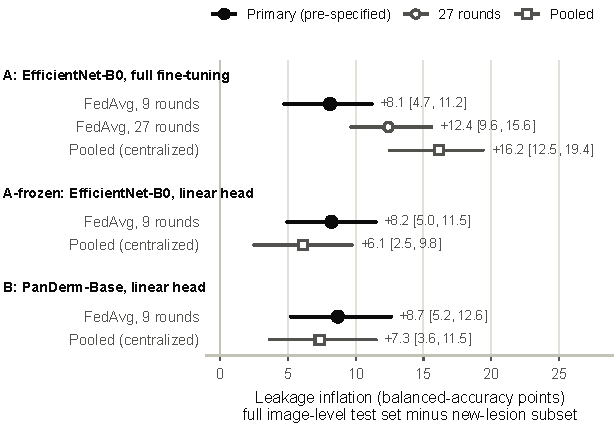
\includegraphics[width=0.62\textwidth]{Fig3_leakage_inflation}
  \caption{Apparent leakage inflation of balanced accuracy (Eq.~\ref{eq:inflation}): BA on the full
  image-level test set minus standardized BA on its new-lesion subset, for the same model (points with
  95\% lesion-bootstrap CI; E1, three seeds). Filled markers: the pre-specified primary FedAvg models.}
  \label{fig:inflation}
\end{figure}

\subsection{Method rankings and accuracy (RQ2, RQ3)}
\label{sec:res-rankings}

Whether leakage changed which method looked best depended on the encoder and the metric
(Figure~\ref{fig:rankings}; Table~\ref{tab:ba}). For model~A and pooled BA, the rankings under the two
split types agreed closely (Kendall's $\tau_b=0.79$, 95\% CI 0.57--0.93), and the agreement of single-seed
rankings across split types (0.66) was close to the seed-to-seed noise floor (0.72). On mean-of-clients
BA, agreement was lower ($\tau_b=0.57$; single-seed 0.24 vs noise floor 0.54), mainly because local-only
training fell from third place on image-level splits to seventh on lesion-grouped splits. For model~B,
rankings on pooled BA were essentially unrelated across split types ($\tau_b=0.05$, $-0.24$ to $0.24$;
single-seed 0.10 vs noise floor 0.74). The FedPer-style two-layer head ranked first on image-level splits
(BA 0.656) and seventh on lesion-grouped splits (0.502). Several of the differences that determine these
ranks are small relative to seed-to-seed variation (Supplementary~S10); for example, model~B FedPer was
2.1 points below FedAvg on lesion-grouped splits (seed range $-5.9$ to $+0.1$). The capacity-matched heads of E9 (Supplementary~S12) indicate that the behaviour of the
FedPer-style head comes from its two-layer architecture rather than from personalization: a FedAvg model
with the same two-layer head showed an apparent inflation of 10.4 points in clients 0, 2 and 3 (FedPer-style
head 10.6, linear FedAvg 6.1) and fell from sixth place on image-level to last place on lesion-grouped
splits (pooled BA 0.606 to 0.466), and the two-layer pooled and local-only heads inflated more than their
linear counterparts (6.4 vs 2.7 and 6.8 vs 4.2 points). With the three two-layer heads added, the agreement
of the model~B rankings across split types remained low ($\tau_b=0.20$, 0.02--0.42; single-seed 0.27 vs
noise floor 0.72).

Pooled BA was lower on lesion-grouped than on image-level test sets for every method and encoder
(Table~\ref{tab:ba}); mean-of-clients BA was not always lower (model~B FedAvg 0.532 vs 0.546). Centralized
pooled training remained best for model~A (pooled BA 0.566). Among the federated methods, FedPer was best
for model~A on pooled BA (0.555, 6.0 points above FedAvg at 0.495; seed range of the difference 1.8 to
10.5), and FedBN on mean-of-clients BA (0.568). For model~B, the federated methods differed by at most
4 points (0.502--0.542), and local-only training reached the highest pooled BA (0.566).

\begin{figure*}[!t]
  \centering
  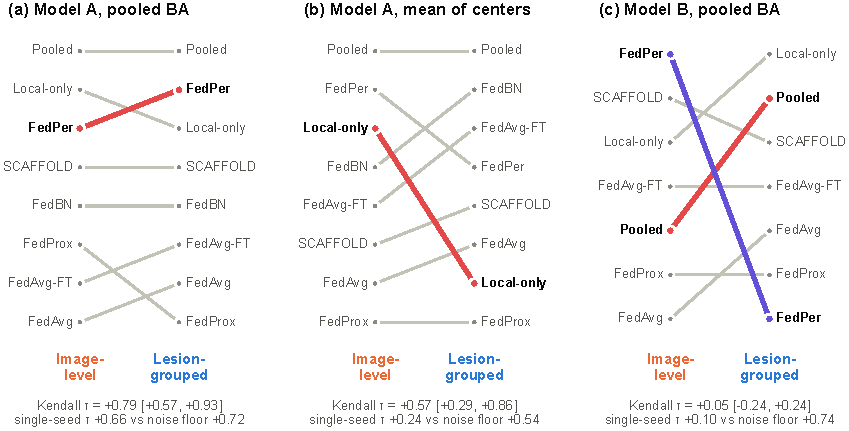
\includegraphics[width=\textwidth]{Fig4_rankings}
  \caption{Method rankings on image-level (left) and lesion-grouped (right) test sets, by mean pooled BA
  over five seeds (top = best). Highlighted methods change rank most. Text below each panel: Kendall's
  $\tau_b$ between the two rankings (95\% CI), and the agreement of single-seed rankings across split types
  compared with the seed-to-seed noise floor.}
  \label{fig:rankings}
\end{figure*}

\inputtable{Table3_balanced_accuracy}

\subsection{Exploratory associations with fitting capacity and feature proximity (RQ3)}
\label{sec:res-mechanism}

In the pre-specified H3b contrast (clients 0, 2 and 3), the local and personalized group of model~A showed
3.2 points more apparent inflation than FedAvg (95\% CI 2.0--4.6; supported), but the difference came
mainly from local-only training (13.7 points) and, to a lesser extent, FedPer (6.7 points); FedBN (4.9) and
FedAvg-FT (4.8) were close to FedAvg (4.3), whereas non-personalized pooled training showed 12.1 points
(Figure~\ref{fig:mechanism}b). For model~B, whose other heads are linear, local-only (4.2) and pooled (2.7)
training showed the least inflation, and the H3b contrast was not supported (0.9 points, $-0.2$ to 2.1).
The FedPer-style two-layer head showed the largest inflation of the model~B methods (10.6 points). These
comparisons span different optimizers, training budgets and head architectures, so they show an
association with how strongly a model fits its training lesions, not a controlled effect of capacity; the
randomized exposure effects of E8 (Section~\ref{sec:res-leakage}) and the capacity-matched heads of E9
(Section~\ref{sec:res-rankings}) order the methods in the same way.

Per-client inflation was larger in clients with more leakage (Figure~\ref{fig:mechanism}a), but this
dose--response is weak evidence. Weighted least-squares slopes ranged from 8.1 points per 100\% leakage
(FedAvg) to 21.5 (local-only) for model~A and from 6.2 to 18.9 for model~B, but client~0 carried most of
the leakage and most of the inflation (10.0 to 22.2 points for model~A), and without client~0 the slopes
ranged from $-2.2$ to 10.0 points for model~A (FedAvg $-1.9$) and from $-1.9$ to 4.1 for model~B
(Supplementary~S3). The slope is also partly built into the measure, because inflation within a class
scales with the leaked share.

An exploratory nearest-neighbor analysis of the frozen embeddings showed why even linear heads can benefit
from leakage (Figure~\ref{fig:mechanism}c; Supplementary Figure~S1). Leaked test images were closer to the
training set than new-lesion images (mean cosine similarity of the centered embeddings to the nearest
training image 0.81 vs 0.75 for A-frozen; 0.85 vs 0.79 for model~B), and for 54\% (A-frozen) and 58\%
(model~B) of the leaked images the nearest training image belonged to the same lesion. A 1-nearest-neighbor
classifier, which fully exploits this proximity, showed 22.7 and 22.4 points of unweighted inflation, and
the linear heads 6.2 and 6.6 points on the same measure. Leaked and new lesions also differ in class and
client composition, so this comparison does not by itself separate proximity from those differences.

\begin{figure*}[!t]
  \centering
  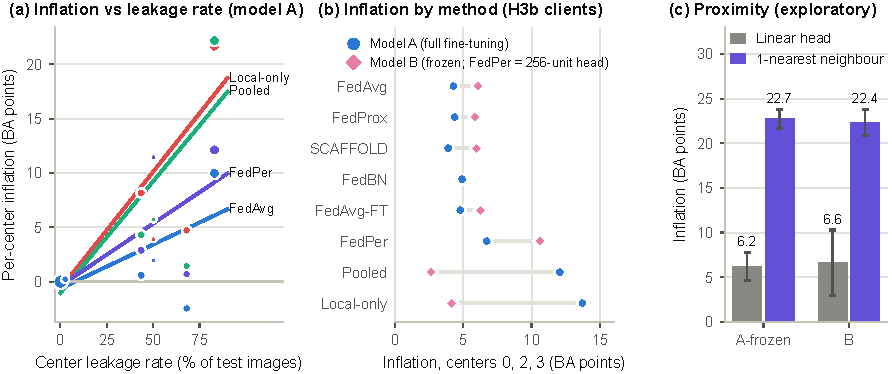
\includegraphics[width=\textwidth]{Fig5_mechanism}
  \caption{Exploratory associations of apparent inflation with leakage rate, method and feature proximity.
  (a) Per-client inflation against the client's leakage rate for four model~A methods, with weighted
  least-squares lines (marker area proportional to the client's new-lesion test images); client~0 carries
  most of the slope (Supplementary~S3). (b) Inflation in clients 0, 2 and 3 (the H3b measure) by method for
  model~A (circles) and model~B (diamonds). (c) Inflation of the frozen-encoder linear heads and of a
  1-nearest-neighbor classifier on the same embeddings (mean $\pm$ SD over seeds; unweighted BA).}
  \label{fig:mechanism}
\end{figure*}

\subsection{Calibration (RQ1, RQ2)}
\label{sec:res-calibration}

Calibration differed more between clients than between methods (Figure~\ref{fig:calibration}). On
lesion-grouped test sets after temperature scaling, the pooled ECE of all methods lay between 0.018 and
0.046 (model~A) and between 0.022 and 0.033 (model~B), whereas per-client ECE ranged from 0.03 to 0.20
and from 0.02 to 0.26. For every method, the highest per-client ECE occurred in client~1 or in the
smallest client~5; part of this spread reflects the finite-sample bias of binned ECE in small clients.

The original E3 analysis compared ECE on the new-lesion subset of each image-level test set with ECE on the
full set and found it higher by 2.9 points (95\% CI 2.5--3.9) for model~A FedAvg and 2.0 points (1.6--2.9)
for model~B FedAvg, which suggested that leaky test sets understate miscalibration. A post hoc sensitivity
analysis did not confirm this (Supplementary~S8). The new-lesion subset is smaller than the full set and
has a different client and class mix, and binned ECE is biased upwards in small samples. Against random
subsets of the full test set with the same size and the same client-by-class counts, the difference
vanished or reversed (model~A FedAvg $-0.5$ points, $-1.0$ to 0.0; model~B FedAvg $-1.0$, $-1.6$ to
$-0.4$; model~A pooled $-2.4$, $-2.8$ to $-1.6$). The bin-free metrics, standardized to the same
composition, were slightly worse on new lesions: NLL by 0.03 (model~A FedAvg), 0.04 (model~B FedAvg) and
0.09 (model~A pooled), and Brier score by 1.0, 1.4 and 3.9 points, mainly reflecting the lower accuracy on
new lesions. Results were similar with 10, 20 or equal-mass bins and after removing the 6.5\% of test
images whose lesion was in the validation fold. Leaky test sets therefore overstated accuracy, but we found
no robust evidence that they understate calibration error as measured by ECE.

Temperatures fitted on lesion-grouped validation data improved ECE on lesion-grouped test sets but worsened
it on image-level test sets for the models that fit their training images most closely
(Figure~\ref{fig:calibration}c): model~A pooled from 0.024 to 0.074, model~A local-only from 0.031 to 0.087,
and the model~B FedPer-style head from 0.066 to 0.085. For the same three models on lesion-grouped test
sets, scaling reduced ECE from 0.052 to 0.018, from 0.094 to 0.019 and from 0.141 to 0.022. These full test
sets have several thousand images, so the comparison is not affected by the small-sample bias. Replacing
the averaged temperature by the NLL-optimal temperature on the pooled validation set changed ECE by at
most 0.8 points (Supplementary~S8). Monte Carlo dropout through the single dropout layer did not
improve on the softmax output in this configuration (raw ECE 0.068 vs 0.065 on image-level and 0.047 vs
0.047 on lesion-grouped test sets).

In a separate descriptive analysis on the image-level test sets, thresholds were calibrated on a random
half of the test lesions and coverage was measured on the other half, separately for leaked and new
evaluation images. Coverage of the two groups differed by at most 1.5 points, and overall coverage was
0.90 for both encoders. This shows that the leaked images did not distort marginal coverage in this
setting; it is not a general robustness guarantee.

\begin{figure*}[!t]
  \centering
  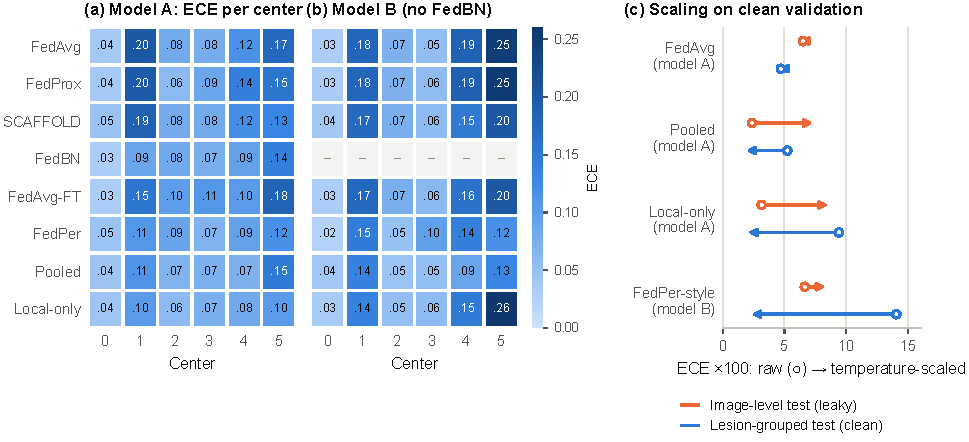
\includegraphics[width=\textwidth]{Fig6_calibration}
  \caption{Calibration. (a, b) Top-label ECE per method and client on lesion-grouped test sets after
  temperature scaling (mean of five seeds; model~B has no FedBN). Values for the small clients 4 and 5 are
  imprecise. (c) ECE ($\times100$) before (open circle) and after temperature scaling fitted on
  lesion-grouped validation data, on image-level (orange) and lesion-grouped (blue) test sets.}
  \label{fig:calibration}
\end{figure*}

\subsection{Federated conformal prediction (RQ1, RQ4)}
\label{sec:res-conformal}

A single global threshold under-covered some clients, as expected for a rule that targets the mixture of
clients, and the pre-specified ShrinkFCP did not fix this (Figure~\ref{fig:conformal};
Table~\ref{tab:conformal}). On the in-federation lesion-grouped FedAvg models (LAC, $\alpha=0.1$), the
global threshold left the worst client at a mean coverage of 0.819 (model~A, client~3) and 0.717 (model~B,
client~4), with worst-client q10 of 0.786 and 0.670; FCP behaved like the global threshold. Client-wise
thresholds gave every client a mean coverage of about 0.90 (worst-client q10 0.794 and 0.795), and the
remaining shortfall in the tail came from the small client~5. ShrinkFCP raised the worst-client q10 of
model~A by 2.5 points over client-wise calibration ($-2.8$ to 3.9) but lowered it by 7.3 points ($-14.0$ to
$-5.4$) for model~B, and for both encoders it violated the mean-coverage guard (lowest client 0.856 and
0.771): RQ4 was not met. The interval for model~A is not centered on the point estimate, because the
bootstrap recomputes q10 from 20 rather than 100 draws per replicate; this is examined below.

On the 18 LOCO models per encoder, the pre-specified test of EB-ShrinkFCP was met for model~A, with a
worst-client q10 of 0.837 against 0.814 for client-wise calibration (gain 2.3 points, 0.8--3.9), set sizes
within 4\% of the reference and every client's mean coverage at least 0.89. The interval supports a gain
above zero, not a gain above 2 points. For model~B the gain was 0.5 points ($-1.7$ to 0.9) and the test was
not met. In all four settings (in-federation and LOCO models, both encoders), EB-ShrinkFCP kept every
client's mean coverage between 0.897 and 0.901, whereas ShrinkFCP dropped the worst client to 0.77--0.86.
On the in-federation models, the post hoc gain of EB-ShrinkFCP over client-wise calibration was 4.8 points
(0.2--6.1) for model~A and 0.1 points for model~B. Per-client set sizes and results for APS scores and for
$\alpha=0.05$ and $0.2$ are given in Supplementary~S5.

Post hoc sensitivity analyses qualify these results (Supplementary~S6). First, q10 estimated from 100 draws
is noisy: for client-wise thresholds on the LOCO models of model~A it ranged from 0.797 to 0.813 across
five independent sets of 100 draws, a spread comparable to the pre-specified gain; with 1,000 draws, the
worst-client q10 was 0.837 for EB-ShrinkFCP and 0.805 for client-wise thresholds (model~A) and 0.805 and
0.797 (model~B). Second, a corrected bootstrap that keeps the resampled copies of a lesion in the same half
gave intervals for the model~A gain over client-wise thresholds of 2.6 to 8.1 points (20 draws per
replicate) and 3.4 to 8.7 (100 draws), and for model~B $-0.3$ to 3.2 and 0.1 to 3.1; these intervals are
not centered on the point estimates, because q10 from resampled clustered data is biased downwards, more
so for the noisier client-wise thresholds. Third, when only one random image per lesion was kept in both
halves, so that calibration and evaluation units are independent lesions, client-wise and EB-ShrinkFCP
thresholds both kept every client's mean coverage at 0.90, and the EB gain in worst-client q10 over
client-wise thresholds was 3.3 points for model~A with an interval that included zero ($-0.4$ to 3.6) and
0.4 points for model~B ($-0.3$ to 1.6); global and FCP thresholds under-covered further (lowest client
0.81 and 0.73). Fourth, when the evaluation half was fixed and only the calibration lesions were redrawn,
EB-ShrinkFCP raised the worst-client q10 over client-wise thresholds by 3.4 points (model~A) and 0.9 points
(model~B), indicating that the gain comes from less variable thresholds rather than from evaluation noise.
Fifth, exact order statistics changed the global and FCP thresholds' q10 by at most 0.003. Finally, the
label-shift-weighted comparator did not repair the per-client shortfall of the global threshold (lowest
client mean coverage 0.85 for model~A and 0.72 for model~B), indicating that the clients differ by more than
their class priors.

On personalized models (FedBN, FedAvg-FT, FedPer and local-only; descriptive), a global threshold still
left some client at a mean coverage of 0.76--0.87, while client-wise thresholds kept every client's mean
coverage between 0.897 and 0.911 and EB-ShrinkFCP between 0.888 and 0.944 (Supplementary~S7).

\begin{figure*}[!t]
  \centering
  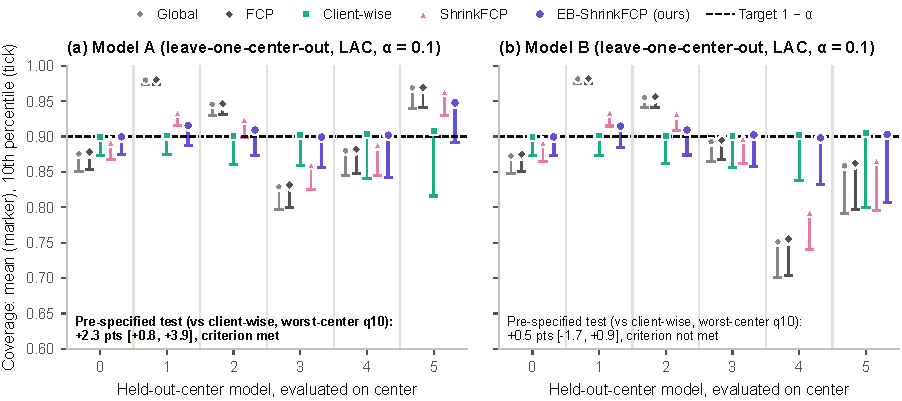
\includegraphics[width=\textwidth]{Fig7_conformal}
  \caption{Federated conformal coverage on LOCO models (LAC, $\alpha=0.1$; 18 models per encoder, 100
  lesion-wise calibration draws each). For each rule and client, the marker is the mean coverage and the
  tick the 10th percentile of coverage over draws (q10), not a confidence interval; dashed line: target
  coverage 0.90. The text gives the pre-specified test of EB-ShrinkFCP against client-wise calibration.}
  \label{fig:conformal}
\end{figure*}

\inputtable{Table4_conformal}

\subsection{Unseen clients and smartphone images (RQ1)}
\label{sec:res-shift}

Accuracy and calibration were worse when a client was unseen in training, and worse still on smartphone
images (Figure~\ref{fig:shift}). On the same held-out test images and seeds, a client held out of training
lost on average 4.6 BA points (model~A) and 5.9 points (model~B) compared with the FedAvg model that
included it; client~0 lost 17.5 and 16.8 points (0.487 to 0.312 and 0.480 to 0.312), and its ECE rose from
0.031 to 0.101 (model~A). For LOCO models, global conformal thresholds left the worst client at a mean
coverage of 0.83 (model~A) and 0.75 (model~B) (Table~\ref{tab:conformal}); because every client, including
the held-out one, was calibrated with its own labelled lesions, client-wise and EB-ShrinkFCP thresholds
reached about 0.90.

On PAD-UFES-20 (closed-set transfer to six shared classes), BA fell from 0.471 on the Fed-ISIC2019
lesion-grouped test set (same six-class restriction) to 0.356 (95\% CI 0.333--0.380) for model~A and from
0.522 to 0.342 (0.320--0.366) for model~B, and ECE rose from 0.058 to 0.190 and from 0.034 to 0.212.
Actinic keratosis, the second most frequent class, was rarely recognized (recall 0.08 and 0.19). Conformal
thresholds transferred from Fed-ISIC2019 covered 0.596 (0.576--0.614) and 0.669 (0.650--0.687) of the
PAD-UFES-20 images instead of 0.90, meeting the pre-specified failure rule; the interval conditions on the
transferred threshold. Recalibrating on half of the PAD-UFES-20 patients restored marginal coverage to
0.900 (10th percentile over draws 0.880 and 0.884), but the prediction sets then contained on average 4.9
(model~A) and 4.3 (model~B) of the six classes, and coverage of actinic keratosis and squamous cell
carcinoma remained between 0.80 and 0.84 (730 and 192 images; about half of each falls in the evaluation half of a draw). The shift combines modality, population, acquisition,
class prevalence and label definitions, so it is not attributable to the imaging device alone.

\begin{figure*}[!t]
  \centering
  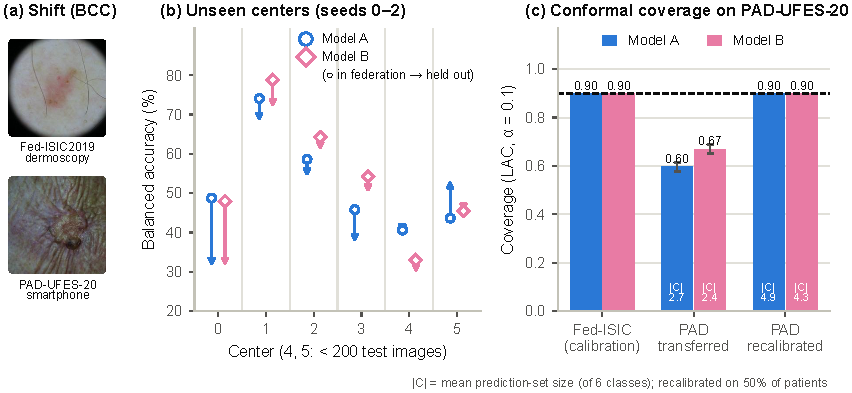
\includegraphics[width=\textwidth]{Fig8_domain_shift}
  \caption{Unseen clients and smartphone images. (a) The same diagnosis (basal cell carcinoma) in a
  Fed-ISIC2019 dermoscopy image and a PAD-UFES-20 smartphone photograph. (b) BA on each client's
  lesion-grouped test set when the client was in the federation (open marker) and when it was held out
  (arrow head); same test images, seeds 0--2. (c) Conformal coverage at $\alpha=0.1$ after the six-class
  restriction: on the Fed-ISIC2019 calibration scores (nominal by construction, shown as reference), on
  PAD-UFES-20 with the transferred threshold (95\% patient-bootstrap CI, conditional on the threshold) and
  after recalibration on 50\% of the patients; $|C|$, mean prediction-set size. Images: ISIC 2019
  (CC-BY-NC 4.0) and PAD-UFES-20 (CC-BY 4.0).}
  \label{fig:shift}
\end{figure*}

% ============================================================== 5. Discussion
\section{Discussion}
\label{sec:discussion}

\subsection{Principal findings}

In Fed-ISIC2019, image-level splitting places sibling images of the same lesion in training and test sets
for 0.1--93\% of each client's test images in the official split. Models looked about 8 balanced-accuracy
points better on the full image-level test sets than on their new-lesion subsets with any of three encoder
configurations, and up to 16 points better for centralized training (RQ2). A randomized experiment on fixed test images confirmed that the sibling images themselves cause this gain (9.1 points for FedAvg) and that it grows with how closely a classifier fits its training lesions. Leakage left the
ranking of fine-tuned methods on the benchmark metric about as stable as re-running with another seed, but
it reordered methods on per-client accuracy and for a foundation-model encoder, where the most flexible
head moved from first to seventh place. The size of the apparent inflation was associated with how closely
a model can fit its training lesions rather than with personalization as such (RQ3). Calibration and
conformal coverage varied more between clients than between methods, and a single global conformal
threshold left some clients well below the target coverage (RQ1). A pre-specified fixed shrinkage rule
failed; an empirical-Bayes variant kept every client's mean coverage near the target and improved the
worst-client tail for one of two encoders (RQ4). Accuracy, calibration and transferred coverage were worse
on unseen clients and much worse on smartphone images.

\subsection{Why leakage inflates apparent accuracy}

Two observations constrain the explanation. First, frozen encoders with linear heads, which have far less
trainable capacity than a fully fine-tuned network, still showed about 8 points of apparent inflation.
Second, inflation was larger for classifiers that fit their training lesions more closely: linear heads
about 6--9 points, the two-layer FedPer-style head about 11, fully fine-tuned networks trained for 20 epochs
12--16, and a 1-nearest-neighbor rule about 22. One explanation consistent with both observations is that
images of one lesion lie close together in feature space, so a test image whose sibling is in training sits
next to a correctly labelled neighbor even in a generic ImageNet embedding, and that how much of this
proximity becomes apparent accuracy depends on how closely the classifier follows individual training
points. This account fits the large inflation of non-personalized pooled training, the small inflation of
FedBN and FedAvg-FT, and the reversal of the local-only advantage between model~A and model~B. The H3b
hypothesis, formulated in terms of personalization, was therefore supported for model~A, but the
supporting difference came mainly from local-only training. Because the capacity comparisons span
different optimizers, budgets and head architectures, and the nearest-neighbor analysis is exploratory,
we regard this as an interpretation, not as a tested causal mechanism. The two additional experiments strengthen this account for the
comparisons they control. In E8, the exposure effect on the same randomized target images ordered the
methods in the same way as the observational contrast (local-only $>$ pooled $>$ FedPer $>$ FedAvg for
model~A; the two-layer head far above the linear heads for model~B), and in E9 a FedAvg model with the
FedPer-style two-layer head inflated as much as the FedPer-style head itself. Head capacity, not the
client-specific layer, therefore explains the behaviour of the FedPer-style head. For the fine-tuned
network, the methods still differ in optimizer and training budget, so fitting capacity remains the most
consistent explanation rather than an isolated cause.

Freezing a foundation model did not remove the apparent inflation: PanDerm showed as much as an ImageNet
encoder under FedAvg, and its most flexible head was the variant most favored by the leaky split. Since
PanDerm's pretraining data are not fully public, some of its specific behavior could reflect overlap with
the evaluation images. The A-frozen control shows that inflation of this size does not require such
overlap, but it does not tell how much of PanDerm's own inflation is due to it.

\subsection{Implications for federated benchmarking}

Differences between FL methods on Fed-ISIC2019 are often a few balanced-accuracy points: in FLamby's
benchmark and in the evaluation of Tavakoli et al., FedAvg, FedProx, SCAFFOLD and personalized methods lie
within about 5 points of each other \cite{flamby2022,tavakoli2024fendafl}. The apparent leakage effect is
of the same size or larger and is unevenly distributed, with most of it in one client. Two consequences
follow. Absolute accuracies reported on image-level splits overstate performance on new lesions, and
leakage can change comparative performance and rankings, with effects that depend on the methods and the
metric. We observed both a benign and a harmful case: for fine-tuned EfficientNet-B0 the pooled ranking was
stable, whereas for frozen PanDerm features it was not. Because the harmful case cannot be recognized
without a grouped split, we recommend lesion- or patient-grouped splits as the default for FL benchmarks
with repeated imaging. This extends previous findings on duplicates and problematic partitions in
centralized dermatology datasets \cite{cassidy2022isic,groger2023reliable,abhishek2025dermamnist} and on
subject-level leakage in other imaging domains \cite{bussola2021tiles,yagis2021leakage} to a federated
benchmark with acquisition-source clients, and to calibration and coverage. The lesion-grouped splits used
here are released with the code.

\subsection{Reliability at the level of the site}

For a clinician, the relevant question is whether probabilities and prediction sets are reliable at their
own site. Four results bear on this. First, pooled ECE values of 0.02--0.05 concealed per-client values up
to 0.26, so pooled calibration metrics are not informative about individual sites, although small clients
also have imprecise ECE. Second, the apparent difference in ECE between new-lesion and full leaky test sets was explained by
sample size and composition; this illustrates that binned ECE should be compared only at matched sample
sizes, and that NLL and Brier score are useful companions. Third, temperature scaling fitted on lesion-grouped validation
lesions made the most strongly fitted models worse on a leaky test set, so calibration studies that tune on
one kind of split and test on another can reach opposite conclusions; validation and test data should be
grouped in the same way. Fourth, a global threshold, including FCP's \cite{lu2023fcp}, targets coverage on
the mixture of clients and under-covered clients whose scores were shifted, whereas client-wise thresholds
were correct on average but noisy in small clients. Client-wise thresholds rest on exchangeability within a
client, which repeated images of one lesion weaken; randomizing whole lesions between calibration and
evaluation and the one-image-per-lesion analysis address this empirically, while hierarchical conformal
methods offer formal guarantees for grouped data \cite{dunn2022hierarchical,lee2023hierarchical}.

EB-ShrinkFCP addresses the noise of client-wise thresholds without returning to a single shared threshold.
Its weight $w_c=\tau^2/(\tau^2+\sigma_c^2)$ estimates from the data how much the clients differ, so it
borrows strength only when they agree; the fixed weight of ShrinkFCP borrowed regardless and imported the
global threshold's bias into the shifted clients. The attainable gain is limited by evaluation noise: with
about 44 evaluation images per draw in the smallest client, even a rule with exactly nominal conditional
coverage has a 10th percentile of observed coverage well below 0.90, although trivial rules such as
returning all classes would reach full coverage at the cost of useless sets. The evidence on RQ4 is
therefore mixed. Across the tested models and clients, EB-ShrinkFCP kept mean client coverage close to the
target; it met its pre-specified criterion on held-out models for model~A, with an interval that excludes
zero but also includes gains below 2 points; no clear improvement was detected for model~B, so the joint criterion
was not met; and class-conditional coverage was not established. The post hoc analyses point the same way but do not strengthen the claim: the gain is visible in the
variability of thresholds, but with one image per lesion its interval includes zero, and its size is
comparable to the Monte Carlo variability of a 100-draw q10. The rule exchanges two
aggregate statistics per client, a quantile and a variance, rather than images or score lists; we did not
analyze its formal privacy properties. Related work on federated conformal prediction has addressed label
shift \cite{plassier2023labelshift}, one-shot aggregation \cite{humbert2023oneshot}, personalization
through localization \cite{min2025pfcp} and group-conditional coverage \cite{wen2026gcfcp}; of these we
compared only a label-shift-weighted threshold.

Under the smartphone-image shift, transferred thresholds lost 23--30 points of coverage, consistent with the
absence of any guarantee under distribution shift \cite{tibshirani2019covariate,barber2023beyond}. Local
recalibration restored marginal coverage only by returning four to five of six classes, and coverage for
actinic keratosis and squamous cell carcinoma stayed below the target. Recalibration can make a model's
uncertainty honest, but it cannot make an unsuitable model useful, and marginal coverage can hide
class-conditional failures \cite{lu2022fair}.

\subsection{Recommendations}

Based on these results, we suggest that federated dermatology studies (i) split data by lesion or patient
and report the leakage rate of any image-level split they compare with; (ii) report balanced accuracy,
calibration and coverage per client, not only pooled, together with the uncertainty of small-client
estimates; (iii) fit temperature and conformal thresholds on data grouped in the same way as the test data;
(iv) state which coverage target a conformal rule serves (mixture, client or class) and compare locally
calibrated and pooled thresholds for that target before adopting a shrinkage rule; (v) evaluate on held-out
clients and, before deployment in a new imaging modality, recalibrate locally and report set sizes and
per-class coverage; and (vi) fix primary analyses in advance and report negative results, in line with
general reporting guidance for clinical prediction models \cite{collins2024tripodai}.

\subsection{Value of a fixed protocol and negative results}

Of the seven pre-specified tests, four were met in full (Gates 1 and 2, the PAD-UFES-20 transfer rule and E8), two were met for one of two encoders (H3b and 5b), and one failed (RQ4). Without a protocol, the failure of ShrinkFCP could have been
followed by adjusting its constant until it succeeded on the same models. Instead, the failure motivated a
new rule that was specified before the held-out models existed and tested on them, and the post hoc results
are labelled as such. The protocol also prevented a selective reading of H3b: the hypothesis was supported
for model~A but not for model~B. The protocol was version-controlled rather than registered externally, and
two amendments were written after results were known (Supplementary~S9); we therefore present the chronology in
full rather than describing the study as pre-registered in the strict sense
\cite{nosek2018preregistration,kapoor2023leakage,varoquaux2022failures}.

\subsection{Limitations}

This study has several limitations. It audits one benchmark whose six clients are acquisition sources,
three of them from one institution; other federated datasets with patient or lesion identifiers are needed
to test generality. Patient identifiers are not available, so different lesions of one patient can fall on
both sides of a lesion-grouped split, and images of one lesion remain correlated within the calibration and
evaluation halves. Clients 4 and 5 have fewer than 200 test images, so their per-client estimates are
imprecise, and much of the leakage effect is driven by client~0. The apparent inflation compares different
groups of test images and can reflect differences in difficulty and multiplicity even after
standardization; the randomized experiment E8 addresses this for lesions with several images, but not for single-image lesions, and its method comparisons still differ in optimizer and budget. Binned ECE is biased in small samples, which affected our original leaky-versus-new
contrast. Three to five seeds limit the precision of ranking comparisons, and the bootstrap intervals
reflect test-sample uncertainty given the trained models, not retraining variability. The pooled and
local-only references use a different optimizer and budget from the federated methods, FedAvg-FT used a
single pre-specified number of fine-tuning steps, and the benchmark clients and test pools were reused
across method development and evaluation. Overlap between PanDerm's pretraining data and the evaluation
images could not be ruled out. Our FedAvg reproduction was 4.2 points below one published value, though
above FLamby's own results. EB-ShrinkFCP met its criterion for one of two encoders, it does not carry a
finite-sample per-client guarantee, and its variance approximation for clustered images is heuristic.
Finally, the mechanism analysis is exploratory.

\subsection{Future work}

Future work should extend the analysis to multi-site datasets with patient identifiers, examine
hierarchical conformal methods that target new patients or lesions directly, compare EB-ShrinkFCP with
personalized, label-shift-aware and group-conditional federated conformal methods
\cite{min2025pfcp,plassier2023labelshift,wen2026gcfcp} under the same coverage target, and target
class-conditional coverage for rare and commonly confused classes.

% ============================================================== 6. Conclusion
\section{Conclusion}
\label{sec:conclusion}

The Fed-ISIC2019 benchmark split places images of the same lesion in training and test sets, unevenly
across its acquisition-source clients. Models look about 8 balanced-accuracy points better on the leaky
test sets than on their new-lesion subsets, and up to 16 points better for centralized training.
In a randomized experiment on fixed test images, which covers lesions with several images, adding sibling
images to training raised balanced accuracy by 9.1 points for FedAvg, with effects between 4.5 and 28.8
points across training regimes. Leakage also changed which methods appeared best, mainly among classifiers
that differed in head architecture or training regime. At the level of individual clients, a shared conformal threshold under-covered some
sites; an empirical-Bayes shrinkage of per-client thresholds kept mean client coverage near the target and
improved the worst-client tail for one of two encoders, while a fixed shrinkage rule failed its
pre-specified test. On unseen clients and smartphone images, reliability dropped further, and local
recalibration restored coverage only with large prediction sets. We recommend that federated medical
imaging benchmarks with repeated imaging use lesion- or patient-grouped splits and report calibration and
coverage per client, and we release the corrected splits, code, predictions and protocol history to
support this.

\bmsection*{Author contributions}
Abu Jafar Sisty: conceptualization, methodology, software, formal analysis, investigation, data
curation, visualization, writing -- original draft. Author Name: Author contributions. Author Name:
Author contributions. Author Name: Author contributions. All authors reviewed and approved the final
manuscript. % TODO: fill in names and roles of authors 2-4

\bmsection*{Acknowledgments}
% TODO: acknowledgments.

\bmsection*{Financial disclosure}
None reported. % TODO: confirm funding

\bmsection*{Conflict of interest}
The authors declare no potential conflict of interests.

\bmsection*{Data availability statement}
Fed-ISIC2019 is available through the FLamby benchmark (ISIC 2019, CC-BY-NC 4.0; HAM10000 under its own
terms) and PAD-UFES-20 from Mendeley Data (doi:10.17632/zr7vgbcyr2.1, CC-BY 4.0). The repository
\url{https://github.com/Sisty37/reliable-fed-derm} contains the split files with SHA-256 checksums and the
script that builds them from the public metadata, the code for training, analysis, tables and figures,
the protocol versions with git tags marking each pre-run state, run logs, the predictions of every model and
all result files, a pinned dependency list (\texttt{requirements-lock.txt}) and the SHA-256 checksums of the
encoder checkpoints and metadata files; frozen-encoder embeddings and PanDerm-derived heads are not redistributed because of the
PanDerm licence. % TODO: archive the submitted version on Zenodo and add its DOI.

\bmsection*{Ethics statement}
This secondary analysis used only publicly available, de-identified datasets under their published
licences; no new data were collected and no patient was contacted. % TODO: add the institutional ethics position if required

\bmsection*{Use of generative AI}
% TODO: state which AI tools were used and for what (for example code assistance and language editing),
% and that the authors reviewed all content and take full responsibility for it.

\bibliography{refs}

\bmsection*{Supporting information}
Supplementary material S1--S17 and Figure S1 are provided as a separate file with this submission.


\end{document}
